\documentclass{article}
% generated by Madoko, version 1.0.3
%mdk-data-line={1}


\usepackage[heading-base={2},section-num={False},bib-label={True}]{madoko2}


\begin{document}



%mdk-data-line={5}
\mdxtitleblockstart{}
%mdk-data-line={5}
\mdxtitle{\mdline{5}实习总结}%mdk
\mdxauthorstart{}
%mdk-data-line={10}
\mdxauthorname{\mdline{10}Claireyyli}%mdk
\mdxauthorend\mdtitleauthorrunning{}{}\mdxtitleblockend%mdk

%mdk-data-line={7}
\section{{\mdfontfamily{Microsoft YaHei}\mdline{7}1.\hspace*{0.5em}\mdline{7}技 术 点}}\label{sec--}%mdk%mdk

%mdk-data-line={8}
\noindent\mdline{8}{\mdfontfamily{Microsoft YaHei}实习期间最直接的收获就是技术上的成长:}\mdline{8}%mdk

%mdk-data-line={9}
\begin{mdbmarginx}{}{}{}{5ex}%mdk
%mdk-data-line={10}
\begin{itemize}[noitemsep,topsep=\mdcompacttopsep]%mdk

%mdk-data-line={10}
\item\mdline{10}Web Audio API%mdk

%mdk-data-line={11}
\item\mdline{11}{\mdfontfamily{Microsoft YaHei} 语音缓存 }\mdline{11}%mdk

%mdk-data-line={12}
\item\mdline{12}{\mdfontfamily{Microsoft YaHei} 语音拼接 }\mdline{12}%mdk

%mdk-data-line={13}
\item\mdline{13}{\mdfontfamily{Microsoft YaHei} 屏幕常亮 }%mdk
%mdk
\end{itemize}%mdk%mdk
\end{mdbmarginx}%mdk

%mdk-data-line={16}
\subsection{\mdline{16}1.1.\hspace*{0.5em}\mdline{16}Web  Audio  API}\label{sec-web-audio-api}%mdk%mdk

%mdk-data-line={17}
\noindent\mdline{17}{\mdfontfamily{Microsoft YaHei}{\mdfontsize{\dimpx{16}}Web Audio API 提供了在Web上控制音频的一个非常有效通用的系统 , 允许开发者来自选音频源,对音频添加作用,创建可视化音频,应用空间效果 (如平移),等等。}}\mdline{17}%mdk

%mdk-data-line={18}
\begin{mdcenter}%mdk

%mdk-data-line={19}
\noindent\mdline{19}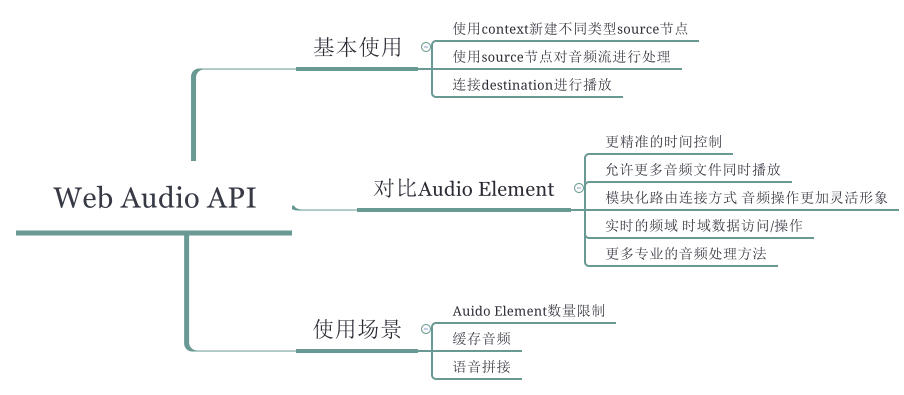
\includegraphics[keepaspectratio=true,width=\dimmin{}{\dimwidth{0.90}}]{images/Web-Audio-API}{}\mdline{19}%mdk
%mdk
\end{mdcenter}%mdk

%mdk-data-line={27}
\begin{mdbmargintb}{}{0.5em}%mdk
\subsection{{\mdfontfamily{Microsoft YaHei}\mdline{27}1.2.\hspace*{0.5em}\mdline{27}缓存}}\label{section}%mdk%mdk
\end{mdbmargintb}%mdk

%mdk-data-line={28}
\begin{itemize}[noitemsep,topsep=\mdcompacttopsep]%mdk

%mdk-data-line={28}
\item\mdline{28}~\mdline{28}indexedDB%mdk

%mdk-data-line={29}
\item\mdline{29}~\mdline{29}localStorage%mdk

%mdk-data-line={30}
\item\mdline{30}~\mdline{30}Service Worker%mdk

%mdk-data-line={31}
\item\mdline{31}~\mdline{31}{\mdfontfamily{Microsoft YaHei}联合使用}\mdline{31}%mdk
%mdk
\end{itemize}%mdk

%mdk-data-line={34}
\begin{mdbmargintb}{}{0.5em}%mdk
\subsubsection{\mdline{34}1.2.1.\hspace*{0.5em}\mdline{34}IndexedDB}\label{sec-indexeddb}%mdk%mdk
\end{mdbmargintb}%mdk

%mdk-data-line={35}
\begin{mdcenter}%mdk

%mdk-data-line={36}
\noindent\mdline{36}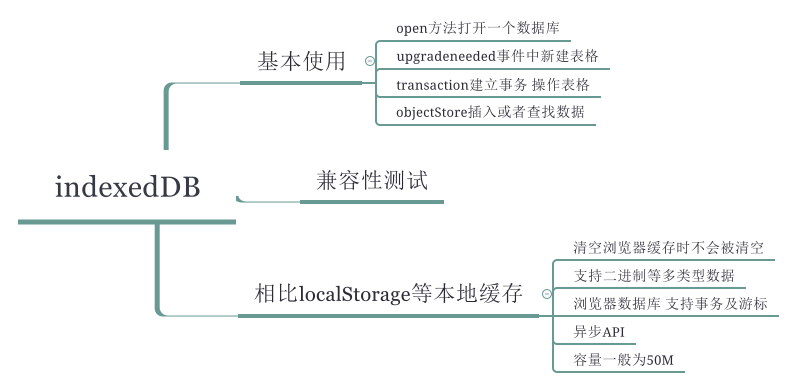
\includegraphics[keepaspectratio=true,width=\dimmin{}{\dimwidth{0.90}}]{images/indexedDB}{}\mdline{36}%mdk
%mdk
\end{mdcenter}%mdk

%mdk-data-line={41}
\begin{mdbmargintb}{}{0.5em}%mdk
\subsubsection{\mdline{41}1.2.2.\hspace*{0.5em}\mdline{41}IndexedDB}\label{sec-indexeddb}%mdk%mdk
\end{mdbmargintb}%mdk

%mdk-data-line={42}
\noindent\mdline{42}{\mdfontfamily{Microsoft YaHei}基本使用}\mdline{42}%mdk
\begin{mdpre}%mdk
\noindent~~~{\mdcolor{darkgreen}//篇幅限制,这里没有展示完整代码}\\
~~\\
~~~{\mdcolor{navy}var}~indexedDB~=~window.indexedDB~\textbar{}\textbar{}~window.webkitIndexedDB~\textbar{}\textbar{}~window.mozIndexedDB;\\
~~~{\mdcolor{navy}var}~request~=~indexedDB.open(dbName,~version);\\
~~~\\
~~~request.onupgradeneeded~=~{\mdcolor{navy}function}(e)\{\\
~~~~{\mdcolor{navy}if}(!db.objectStoreNames.contains(storeName))\{\\
~~~~~~~store~=~db.createObjectStore(storeName);\\
~~~~\}\\
~~~\};\\
~~~\\
~~~{\mdcolor{darkgreen}//~增加/修改一条记录}\\
~~~{\mdcolor{navy}var}~transaction~=~db.transaction({\mdcolor{navy}this}.storeName,~{\mdcolor{maroon}'}{\mdcolor{maroon}readwrite}{\mdcolor{maroon}'});\\
~~~{\mdcolor{navy}var}~objectStore~=~transaction.objectStore({\mdcolor{navy}this}.storeName);\\
~~~{\mdcolor{navy}var}~request~=~objectStore.put(value,~key);\\
~~~{\mdcolor{darkgreen}//~查询一条记录}\\
~~~request~=~objectStore.get(key);\\
~~~{\mdcolor{darkgreen}//~删除一条记录}\\
~~~request~=~objectStore({\mdcolor{navy}this}.storeName).{\mdcolor{navy}delete}(key);\\
~~~{\mdcolor{darkgreen}//~关闭数据库}\\
~~~db.close();%mdk
\end{mdpre}
%mdk-data-line={68}
\begin{mdbmargintb}{}{0.5em}%mdk
\subsubsection{\mdline{68}1.2.3.\hspace*{0.5em}\mdline{68}IndexedDB}\label{sec-indexeddb}%mdk%mdk
\end{mdbmargintb}%mdk

%mdk-data-line={69}
\noindent\mdline{69}{\mdfontfamily{Microsoft YaHei}兼容性测试}\mdline{69}%mdk

%mdk-data-line={70}
\begin{mdcenter}%mdk

%mdk-data-line={71}
\noindent\mdline{71}\includegraphics[keepaspectratio=true,width=\dimmin{}{\dimwidth{0.90}}]{images/indexedDB-}{}\mdline{71}%mdk
%mdk
\end{mdcenter}%mdk

%mdk-data-line={76}
\begin{mdbmargintb}{}{0.5em}%mdk
\subsubsection{\mdline{76}1.2.4.\hspace*{0.5em}\mdline{76}localStorage}\label{sec-localstorage}%mdk%mdk
\end{mdbmargintb}%mdk

%mdk-data-line={77}
\begin{mdcenter}%mdk

%mdk-data-line={78}
\noindent\mdline{78}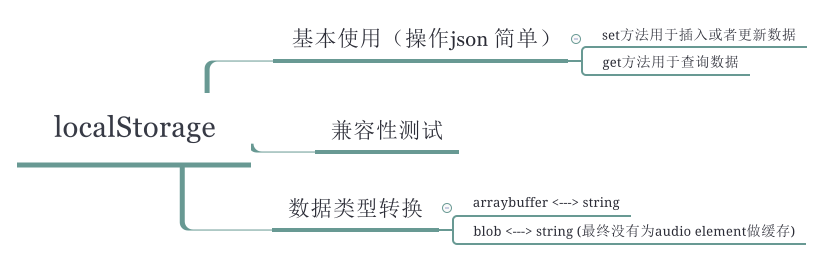
\includegraphics[keepaspectratio=true,width=\dimmin{}{\dimwidth{0.90}}]{images/localStorage}{}\mdline{78}%mdk
%mdk
\end{mdcenter}%mdk

%mdk-data-line={83}
\noindent\mdline{83}{\mdfontfamily{Microsoft YaHei}{\mdfontsize{\dimpx{14}}{\mdcolor{\#AAAAAA}基本使用很简单,不再赘述}}}\mdline{83}%mdk

%mdk-data-line={86}
\begin{mdbmargintb}{}{0.5em}%mdk
\subsubsection{\mdline{86}1.2.5.\hspace*{0.5em}\mdline{86}localStorage}\label{sec-localstorage}%mdk%mdk
\end{mdbmargintb}%mdk

%mdk-data-line={87}
\noindent\mdline{87}{\mdfontfamily{Microsoft YaHei}兼容性测试}\mdline{87}%mdk

%mdk-data-line={88}
\begin{mdcenter}%mdk

%mdk-data-line={89}
\noindent\mdline{89}\includegraphics[keepaspectratio=true,width=\dimmin{}{\dimwidth{0.90}}]{images/localStorage-}{}\mdline{89}%mdk
%mdk
\end{mdcenter}%mdk

%mdk-data-line={92}
\noindent\mdline{92}{\mdfontfamily{Microsoft YaHei}{\mdfontsize{\dimpx{14}}{\mdcolor{\#AAAAAA}?表示部分支持}}}\mdline{92}%mdk

%mdk-data-line={95}
\begin{mdbmargintb}{}{0.5em}%mdk
\subsubsection{\mdline{95}1.2.6.\hspace*{0.5em}\mdline{95}localStorage}\label{sec-localstorage}%mdk%mdk
\end{mdbmargintb}%mdk

%mdk-data-line={96}
\noindent\mdline{96}{\mdfontfamily{Microsoft YaHei}数据类型转换}\mdline{96}%mdk
\begin{mdpre}%mdk
\noindent~{\mdcolor{navy}function}~ab2str(buf)~\{\\
~~~~{\mdcolor{navy}var}~uint8array~=~{\mdcolor{navy}new}~Uint8Array(buf);\\
~~~~{\mdcolor{navy}var}~result~=~{\mdcolor{maroon}'}{\mdcolor{maroon}'};\\
~~~~{\mdcolor{navy}for}({\mdcolor{navy}var}~i={\mdcolor{purple}0};~i\textless{}uint8array.length;~i++)\{\\
~~~~~~~~result~+=~String.fromCharCode.apply({\mdcolor{navy}null},~uint8array.slice(i,~i+{\mdcolor{purple}1}));\\
~~~~\}\\
~~~~{\mdcolor{navy}return}~result;\\
~\}\\
~\\
~{\mdcolor{navy}function}~str2ab(str)~\{\\
~~~~{\mdcolor{navy}var}~buf~=~{\mdcolor{navy}new}~ArrayBuffer(str.length);\\
~~~~{\mdcolor{navy}var}~bufView~=~{\mdcolor{navy}new}~Uint8Array(buf);\\
~~~~{\mdcolor{navy}for}~({\mdcolor{navy}var}~i={\mdcolor{purple}0},~strLen=str.length;~i\textless{}strLen;~i++)~\{\\
~~~~~~~~bufView{}[i]~=~str.charCodeAt(i);\\
~~~~\}\\
~~~~{\mdcolor{navy}return}~buf;\\
~\}%mdk
\end{mdpre}
%mdk-data-line={118}
\begin{mdbmargintb}{}{0.5em}%mdk
\subsubsection{\mdline{118}1.2.7.\hspace*{0.5em}\mdline{118}Service  Worker}\label{sec-service-worker}%mdk%mdk
\end{mdbmargintb}%mdk

%mdk-data-line={119}
\begin{mdcenter}%mdk

%mdk-data-line={120}
\noindent\mdline{120}\includegraphics[keepaspectratio=true,width=\dimmin{}{\dimwidth{0.90}}]{images/Service-Worker}{}\mdline{120}%mdk
%mdk
\end{mdcenter}%mdk

%mdk-data-line={125}
\begin{mdbmargintb}{}{0.5em}%mdk
\subsubsection{\mdline{125}1.2.8.\hspace*{0.5em}\mdline{125}Service  Worker}\label{sec-service-worker}%mdk%mdk
\end{mdbmargintb}%mdk

%mdk-data-line={126}
\noindent\mdline{126}{\mdfontfamily{Microsoft YaHei}基本使用}\mdline{126}%mdk
\begin{mdpre}%mdk
\noindent~~{\mdcolor{darkgreen}//~篇幅限制,这里展示的是拦截请求并返回模拟响应}\\
~~\\
~~~self.addEventListener({\mdcolor{maroon}'}{\mdcolor{maroon}fetch}{\mdcolor{maroon}'},~{\mdcolor{navy}function}(e)\{\\
~~~~{\mdcolor{navy}var}~sourceType~=~e.request.url\\
~~~~~~~~~~~~~~~~~~~~~~.split({\mdcolor{maroon}'}{\mdcolor{maroon}.}{\mdcolor{maroon}'}){}[e.request.url.split({\mdcolor{maroon}'}{\mdcolor{maroon}.}{\mdcolor{maroon}'}).length-{\mdcolor{purple}1}].toLowerCase();\\
~~~~{\mdcolor{navy}if}(sourceType~===~{\mdcolor{maroon}'}{\mdcolor{maroon}mp3}{\mdcolor{maroon}'})\{\\
~~~~~~~~~e.respondWith(caches.match(e.request).then({\mdcolor{navy}function}(response)\{\\
~~~~~~~~~~~~{\mdcolor{navy}if}(response)\{\\
~~~~~~~~~~~~~~~~{\mdcolor{navy}return}~response;\\
~~~~~~~~~~~~\}{\mdcolor{navy}else}\{\\
~~~~~~~~~~~~~~~~fetch(e.request).then({\mdcolor{navy}function}(response)\{\\
~~~~~~~~~~~~~~~~~~~~caches.open(CACHE\_VERSION).then({\mdcolor{navy}function}(cache)\{\\
~~~~~~~~~~~~~~~~~~~~~~~~cache.put(e.request,~response.clone());\\
~~~~~~~~~~~~~~~~~~~~\}).then({\mdcolor{navy}function}()\{\\
~~~~~~~~~~~~~~~~~~~~~~~~{\mdcolor{navy}return}~response;\\
~~~~~~~~~~~~~~~~~~~~\});\\
~~~~~~~~~~~~~~~~\});\\
~~~~~~~~~~~~\}\\
~~~~~~~~\}));\\
~~~~\}{\mdcolor{navy}else}\{\\
~~~~~~~~console.log({\mdcolor{maroon}'}{\mdcolor{maroon}Fetched~file~is~not~mp3}{\mdcolor{maroon}'},~sourceType);\\
~~~~\}\\
\});%mdk
\end{mdpre}
%mdk-data-line={154}
\begin{mdbmargintb}{}{0.5em}%mdk
\subsubsection{\mdline{154}1.2.9.\hspace*{0.5em}\mdline{154}Service  Worker}\label{sec-service-worker}%mdk%mdk
\end{mdbmargintb}%mdk

%mdk-data-line={155}
\noindent\mdline{155}{\mdfontfamily{Microsoft YaHei}兼容性测试}\mdline{155}%mdk

%mdk-data-line={156}
\begin{mdcenter}%mdk

%mdk-data-line={157}
\noindent\mdline{157}\includegraphics[keepaspectratio=true,width=\dimmin{}{\dimwidth{0.90}}]{images/serviceWorker-}{}\mdline{157}%mdk
%mdk
\end{mdcenter}%mdk

%mdk-data-line={162}
\noindent\mdline{162}{\mdfontfamily{Microsoft YaHei}{\mdfontsize{\dimpx{16}}{\mdcolor{\#AAAAAA}Android上QQ浏览器可以注册worker,但是install、active事件不触发,控制台报错:The Service Worker security policy prevented an action}}}\mdline{162}%mdk

%mdk-data-line={165}
\begin{mdbmargintb}{}{0.5em}%mdk
\subsubsection{{\mdfontfamily{Microsoft YaHei}\mdline{165}1.2.10.\hspace*{0.5em}\mdline{165}联合使用}}\label{section}%mdk%mdk
\end{mdbmargintb}%mdk

%mdk-data-line={166}
\begin{itemize}[noitemsep,topsep=\mdcompacttopsep]%mdk

%mdk-data-line={166}
\item\mdline{166}{\mdfontfamily{Microsoft YaHei}优先级确定}\mdline{166}%mdk

%mdk-data-line={167}
\item\mdline{167}{\mdfontfamily{Microsoft YaHei}流程图}\mdline{167}%mdk
%mdk
\end{itemize}%mdk

%mdk-data-line={170}
\begin{mdbmargintb}{}{0.5em}%mdk
\paragraph{{\mdfontfamily{Microsoft YaHei}\mdline{170}优先级确定}}\label{section}%mdk%mdk
\end{mdbmargintb}%mdk

%mdk-data-line={171}
\begin{mdcenter}%mdk

%mdk-data-line={172}
\noindent\mdline{172}\includegraphics[keepaspectratio=true,width=\dimmin{}{\dimwidth{0.90}}]{images/pc-}{}\mdline{172}%mdk
%mdk
\end{mdcenter}%mdk

%mdk-data-line={177}
\begin{mdbmargintb}{}{0.5em}%mdk
\paragraph{{\mdfontfamily{Microsoft YaHei}\mdline{177}优先级确定}}\label{section}%mdk%mdk
\end{mdbmargintb}%mdk

%mdk-data-line={178}
\begin{mdcenter}%mdk

%mdk-data-line={179}
\noindent\mdline{179}\includegraphics[keepaspectratio=true,width=\dimmin{}{\dimwidth{0.90}}]{images/phone-}{}\mdline{179}%mdk
%mdk
\end{mdcenter}%mdk

%mdk-data-line={184}
\begin{mdbmargintb}{}{0.5em}%mdk
\paragraph{{\mdfontfamily{Microsoft YaHei}\mdline{184}优先级确定}}\label{section}%mdk%mdk
\end{mdbmargintb}%mdk

%mdk-data-line={185}
\noindent\mdline{185}{\mdfontfamily{Microsoft YaHei}根据兼容性和性能测试结果:}\mdline{185}%mdk

%mdk-data-line={186}
\begin{mdbmarginx}{}{}{}{5ex}%mdk
%mdk-data-line={187}
\begin{itemize}[noitemsep,topsep=\mdcompacttopsep]%mdk

%mdk-data-line={187}
\item\mdline{187}{\mdfontfamily{Microsoft YaHei}{\mdfontsize{\dimpx{16}}速度:indexedDB/localStorage优于service worker,故仅使用service worker做缓存版本控制}}\mdline{187}%mdk

%mdk-data-line={188}
\item\mdline{188}{\mdfontfamily{Microsoft YaHei}{\mdfontsize{\dimpx{16}}兼容性:localStorage优于indexedDB,但indexedDB可以直接缓存二进制文件,故优先使用indexedDB}}%mdk
%mdk
\end{itemize}%mdk%mdk
\end{mdbmarginx}%mdk

%mdk-data-line={192}
\begin{mdbmargintb}{}{0.5em}%mdk
\paragraph{{\mdfontfamily{Microsoft YaHei}\mdline{192}流程图}}\label{section}%mdk%mdk
\end{mdbmargintb}%mdk

%mdk-data-line={193}
\begin{mdcenter}%mdk

%mdk-data-line={194}
\noindent\mdline{194}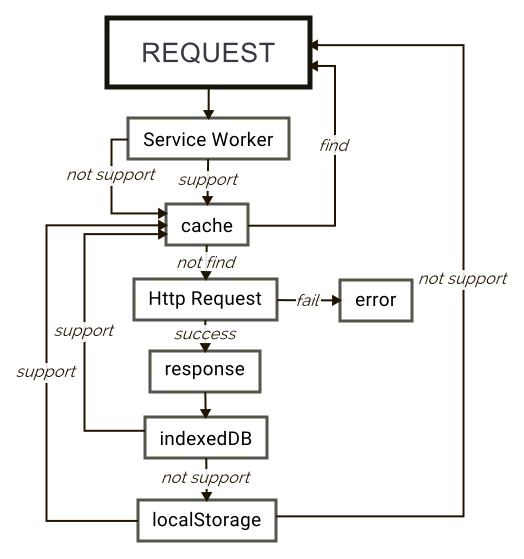
\includegraphics[keepaspectratio=true,width=\dimmin{}{\dimwidth{0.90}}]{images/request}{}\mdline{194}%mdk
%mdk
\end{mdcenter}%mdk

%mdk-data-line={197}
\noindent\mdline{197}{\mdfontfamily{Microsoft YaHei}{\mdfontsize{\dimpx{14}}{\mdcolor{\#AAAAAA}一次上线所有缓存策略风险较大,第一期缓存使用兼容性较好的localStorage进行}}}\mdline{197}%mdk

%mdk-data-line={200}
\begin{mdbmargintb}{}{0.5em}%mdk
\subsection{{\mdfontfamily{Microsoft YaHei}\mdline{200}1.3.\hspace*{0.5em}\mdline{200}语 音 拼 接}}\label{sec--}%mdk%mdk
\end{mdbmargintb}%mdk

%mdk-data-line={201}
\begin{mdcenter}%mdk

%mdk-data-line={202}
\noindent\mdline{202}\includegraphics[keepaspectratio=true,width=\dimmin{}{\dimwidth{0.90}}]{images/aucombo-}{}\mdline{202}%mdk
%mdk
\end{mdcenter}%mdk

%mdk-data-line={207}
\begin{mdbmargintb}{}{0.5em}%mdk
\subsection{{\mdfontfamily{Microsoft YaHei}\mdline{207}1.4.\hspace*{0.5em}\mdline{207}语 音 拼 接}}\label{sec--}%mdk%mdk
\end{mdbmargintb}%mdk

%mdk-data-line={208}
\noindent\mdline{208}{\mdfontfamily{Microsoft YaHei}兼容性测试}\mdline{208}%mdk

%mdk-data-line={209}
\begin{mdcenter}%mdk

%mdk-data-line={210}
\noindent\mdline{210}\includegraphics[keepaspectratio=true,width=\dimmin{}{\dimwidth{0.90}}]{images/http-}{}\mdline{210}%mdk
%mdk
\end{mdcenter}%mdk

%mdk-data-line={217}
\begin{mdbmargintb}{}{0.5em}%mdk
\subsection{{\mdfontfamily{Microsoft YaHei}\mdline{217}1.5.\hspace*{0.5em}\mdline{217}语 音 拼 接}}\label{sec--}%mdk%mdk
\end{mdbmargintb}%mdk

%mdk-data-line={218}
\noindent\mdline{218}{\mdfontfamily{Microsoft YaHei}兼容性测试}\mdline{218}%mdk

%mdk-data-line={219}
\begin{mdcenter}%mdk

%mdk-data-line={220}
\noindent\mdline{220}\includegraphics[keepaspectratio=true,width=\dimmin{}{\dimwidth{0.90}}]{images/ls-}{}\mdline{220}%mdk
%mdk
\end{mdcenter}%mdk

%mdk-data-line={225}
\begin{mdbmargintb}{}{0.5em}%mdk
\subsection{{\mdfontfamily{Microsoft YaHei}\mdline{225}1.6.\hspace*{0.5em}\mdline{225}语 音 拼 接}}\label{sec--}%mdk%mdk
\end{mdbmargintb}%mdk

%mdk-data-line={226}
\noindent\mdline{226}{\mdfontfamily{Microsoft YaHei}兼容性测试}\mdline{226}%mdk

%mdk-data-line={227}
\begin{mdcenter}%mdk

%mdk-data-line={228}
\noindent\mdline{228}\includegraphics[keepaspectratio=true,width=\dimmin{}{\dimwidth{0.90}}]{images/pj-}{}\mdline{228}%mdk
%mdk
\end{mdcenter}%mdk

%mdk-data-line={233}
\begin{mdbmargintb}{}{0.5em}%mdk
\subsection{{\mdfontfamily{Microsoft YaHei}\mdline{233}1.7.\hspace*{0.5em}\mdline{233}语 音 拼 接}}\label{sec--}%mdk%mdk
\end{mdbmargintb}%mdk

%mdk-data-line={234}
\begin{itemize}[noitemsep,topsep=\mdcompacttopsep]%mdk

%mdk-data-line={234}
\item\mdline{234}{\mdfontfamily{Microsoft YaHei}{\mdfontsize{\dimpx{16}}audio element拼接兼容性较差,目前不考虑其拼接}}\mdline{234}%mdk

%mdk-data-line={235}
\item\mdline{235}{\mdfontfamily{Microsoft YaHei}{\mdfontsize{\dimpx{16}}web audio api拼接方案中,拼接数据源再播放兼容性较差,使用先后播放方案进行拼接}}\mdline{235}%mdk
%mdk
\end{itemize}%mdk

%mdk-data-line={238}
\begin{mdbmargintb}{}{0.5em}%mdk
\subsection{{\mdfontfamily{Microsoft YaHei}\mdline{238}1.8.\hspace*{0.5em}\mdline{238}屏 幕 常 亮}}\label{sec--}%mdk%mdk
\end{mdbmargintb}%mdk

%mdk-data-line={239}
\begin{mdcenter}%mdk

%mdk-data-line={240}
\noindent\mdline{240}\includegraphics[keepaspectratio=true,width=\dimmin{}{\dimwidth{0.90}}]{images/cl-}{}\mdline{240}%mdk
%mdk
\end{mdcenter}%mdk

%mdk-data-line={243}
\noindent\mdline{243}{\mdfontfamily{Microsoft YaHei}{\mdfontsize{\dimpx{28}}最终没有解决ios下屏幕常亮问题}}\mdline{243}%mdk

%mdk-data-line={246}
\begin{mdbmargintb}{}{0.5em}%mdk
\section{{\mdfontfamily{Microsoft YaHei}\mdline{246}2.\hspace*{0.5em}\mdline{246}方案设计}}\label{section}%mdk%mdk
\end{mdbmargintb}%mdk

%mdk-data-line={247}
\begin{mdcenter}%mdk

%mdk-data-line={248}
\noindent\mdline{248}\includegraphics[keepaspectratio=true,width=\dimmin{}{\dimwidth{0.90}}]{images/design-}{}\mdline{248}%mdk
%mdk
\end{mdcenter}%mdk

%mdk-data-line={253}
\section{\mdline{253}3.\hspace*{0.5em}\mdline{253}hello}\label{sec-hello}%mdk%mdk%mdk


\end{document}
